% Draft manuscript. Target: The Journal of Physical Chemistry A (achemso class).
% Build: latexmk -pdf main.tex   (figures: python paper/make_figures.py from the repo root)
% Items marked \todo{...} need data or a decision before submission.
\documentclass[journal=jpcafh,manuscript=article]{achemso}

\usepackage{amssymb}
\usepackage[version=4]{mhchem}
\usepackage{siunitx}
\usepackage{booktabs}
\usepackage{graphicx}
\usepackage{xcolor}
\usepackage{amsmath}
\newcommand{\todo}[1]{\textcolor{red}{[TODO: #1]}}
\newcommand{\kisc}{k_\mathrm{ISC}}
\newcommand{\Hso}{\hat H_\mathrm{SO}}

\author{Parfait Atchade-Adelomou}
\affiliation[MIT Media Lab]{City Science, MIT Media Lab, Massachusetts Institute of Technology,
  75 Amherst St, Cambridge, MA 02139, USA}
\email{parfait@mit.edu}

\title[Quantum algorithms for photosensitizer screening: an experimental benchmark]
{What Does a Fault-Tolerant Quantum Algorithm Add to Photosensitizer Screening?
 An Experimental Benchmark of Absorption and Intersystem Crossing in BODIPY Dyes}

\abbreviations{PDT, ISC, SOC, QSVT, CAS, MLJ}
\keywords{photodynamic therapy, BODIPY, intersystem crossing, quantum algorithms, QSVT, TDDFT}

\begin{document}

\begin{tocentry}
\todo{TOC graphic}
\end{tocentry}

% ---------------------------------------------------------------------------------------------
\begin{abstract}
A recent proposal describes fault-tolerant quantum algorithms to screen photosensitizers for
photodynamic therapy (PDT) through two observables computed in a molecular active space: the
dipole spectral weight inside a therapeutic absorption window, obtained by quantum singular value
transformation (QSVT), and an intersystem crossing (ISC) proxy obtained from short-time evolution
under the spin--orbit Hamiltonian. We ask what these observables would contribute to a screening
campaign, by comparing them with an inexpensive classical pipeline and with experiment on a set of
boron-dipyrromethene (BODIPY) dyes with measured photophysics. The classical pipeline (GFN2-xTB
geometries, B3LYP/def2-SVP, $\Delta$SCF correction of S$_1$ and T$_1$, a one-electron spin--orbit
operator calibrated on atomic spin--orbit constants, and Marcus--Levich--Jortner rates) reproduces
the absorption maxima of six dyes with a mean error of $-0.055$~eV (standard deviation 0.02~eV) and
the heavy-atom enhancement of ISC, with $\kisc$ of the di- and tri-iodinated dyes within a factor of
two of experiment. It does not transfer to three $\pi$-extended distyryl dyes: their absorption is
predicted 0.21--0.23~eV too low and the triplet yield of the diiodo derivative 0.04 instead of
0.76, because the $\Delta$SCF correction overshoots and closes a near-resonant S$_1\to$T$_2$
channel. We implemented both quantum algorithms in PennyLane and verified them against
exact diagonalization in small active spaces. Their accuracy, however, is bounded by the active-space
Hamiltonian they act on: at the paper-sized (12e,11o) active space, CASCI places S$_1$ 1.4--2.0~eV
above experiment, and SC-NEVPT2 reduces the error to 0.06--0.27~eV with a sign that varies across
dyes, so an exact quantum solution of the CASCI problem would not improve on the classical
predictions for absorption. The ISC proxy orders the dyes correctly by heavy-atom content but
contains no singlet--triplet energy gap and so cannot identify which triplet channel is open. A
fault-tolerant resource estimate for the (12e,11o) problem gives about 600 logical qubits and
$4\times10^{7}$ Toffoli gates per phase-estimation run. We conclude that, for this class of
molecules, the bottleneck is dynamic correlation and vibronic physics rather than the static
correlation that quantum phase estimation targets, and we outline where quantum algorithms could
still contribute.
\end{abstract}

% ---------------------------------------------------------------------------------------------
\section{Introduction}

Photodynamic therapy relies on a photosensitizer that absorbs light in the tissue-transparent
window (roughly 650--850~nm), undergoes intersystem crossing to its lowest triplet state, and
transfers energy to molecular oxygen to produce cytotoxic singlet oxygen~\cite{Agostinis2011}.
A useful photosensitizer must therefore combine strong red absorption, efficient ISC and a triplet
energy above that of \ce{O2}($^1\Delta_g$), 0.98~eV. Boron-dipyrromethene (BODIPY) dyes are a
common scaffold: they absorb strongly, their absorption can be shifted to the red by aza
substitution or $\pi$-extension, and ISC can be switched on by heavy atoms such as iodine at the
2,6 positions~\cite{Loudet2007,Kamkaew2013}.

Zhou \emph{et al.}~\cite{Zhou2025} recently proposed fault-tolerant quantum algorithms to screen
such photosensitizers. Absorption in the therapeutic window is cast as a threshold projection:
the dipole-excited state $\hat\mu\lvert\Psi_0\rangle$ is filtered with a QSVT polynomial that
approximates the indicator function of the window, and the success probability gives the dipole
spectral weight inside it. ISC is estimated with an evolution proxy,
$\lvert\langle \mathrm{T},M\rvert e^{-i\Hso t}\lvert \mathrm{S}_1\rangle\rvert^2$, which at short
times is proportional to the squared spin--orbit coupling (SOC) matrix element. The authors applied
the approach to BODIPY derivatives and estimated that active spaces of 11--45 spatial orbitals would
require roughly 180--350 logical qubits and Toffoli depths of $10^{7}$--$10^{9}$.

That work is a resource and algorithm study; it does not compare the predicted observables with
measured photophysics. Before quantum hardware for such calculations exists, it is useful to know
whether the proposed observables, evaluated exactly, would rank photosensitizers correctly, and how
they compare with what a classical calculation already provides at low cost. This is the question
we address. We do not propose a new method. Instead, we

\begin{enumerate}
  \item assemble a classical screening pipeline from standard components and validate it against
        absorption maxima, singlet--triplet gaps and ISC rates measured for BODIPY dyes;
  \item implement the two quantum algorithms of ref~\citenum{Zhou2025} in PennyLane, verify them
        against exact results in small active spaces, and evaluate them on the same dyes;
  \item compute classical CASCI and SC-NEVPT2 references in the (12e,11o) active space, which
        bound what an exact quantum solver of the active-space problem could deliver; and
  \item estimate fault-tolerant resources for that active space with the same tools.
\end{enumerate}

The code, input geometries and all results are openly available (Data Availability).

% ---------------------------------------------------------------------------------------------
\section{Methods}

\subsection{Classical pipeline}

\paragraph{Geometries.} Structures are generated from SMILES with RDKit and MMFF94~\cite{Halgren1996}
and optimized with GFN2-xTB~\cite{Bannwarth2019} (tblite, via ASE). E/Z labels are given explicitly
for styryl C=C bonds and the resulting geometries are checked to be trans (see
Section~\ref{sec:styryl}). One conformer is used, in the gas phase.

\paragraph{Excited states.} Ground states are computed with B3LYP~\cite{Becke1993,Stephens1994}/def2-SVP%
~\cite{Weigend2005} in PySCF~\cite{Sun2020} with density fitting and an effective core potential for
iodine. Singlet excitations are obtained by full TDDFT (random-phase approximation) with an
in-house Davidson solver in the Stratmann--Scuseria--Frisch formulation~\cite{Stratmann1998},
restricted to an orbital-energy window of 60~eV; triplets are obtained by the Tamm--Dancoff
approximation in a 10~eV window. For the 60-atom aza-BODIPY we checked that reducing the singlet
window to 25~eV changes S$_1$ by less than $10^{-9}$~eV.

\paragraph{$\Delta$SCF correction.} TDDFT is known to overestimate the S$_1$ energy of
cyanine-like chromophores such as BODIPY by several tenths of an eV~\cite{Momeni2015,LeGuennic2015}.
We therefore replace the TDDFT S$_1$ and T$_1$ energies with $\Delta$SCF values: T$_1$ from an
unrestricted $M_S=1$ calculation, and S$_1$ from the spin-purified sum rule
$E(\mathrm{S}_1)=2E(\mathrm{M})-E(\mathrm{T}_1)$~\cite{Ziegler1977}, where M is a mixed
open-shell determinant converged with the maximum-overlap method~\cite{Gilbert2008}. Higher
singlets and triplets retain their TDDFT energies.

\paragraph{Spin--orbit coupling.} We use an effective one-electron spin--orbit operator built from
the atomic $\hat l/r^3$ integrals, with one scale factor per element chosen so that the isolated
atom, in the same basis and with the same ECP, reproduces the experimental valence spin--orbit
constant $\zeta_{np}$ (e.g.\ \SI{28}{cm^{-1}} for C, \SI{5069}{cm^{-1}} for I). This is equivalent in
spirit to effective nuclear charges~\cite{Koseki1992}; for C, N and F the calibrated effective
charges come out close to the usual values without being imposed. Matrix elements
$V_n=\bigl(\sum_M \lvert\langle \mathrm{S}_1\rvert\Hso\lvert\mathrm{T}_n,M\rangle\rvert^2\bigr)^{1/2}$
are evaluated from the TDA amplitudes. As a sanity check, the operator reproduces the El-Sayed
selection rules~\cite{ElSayed1963} in formaldehyde.

\paragraph{Rates.} The ISC rate is computed with the Fermi golden rule and a
Marcus--Levich--Jortner (MLJ) Franck--Condon weighted density of states~\cite{Jortner1976},
summed over all triplets below and above S$_1$:
\begin{equation}
  \kisc = \sum_n \frac{2\pi}{\hbar} V_n^2
  \sum_{v=0}^{\infty} \frac{e^{-S}S^v}{v!}
  \frac{1}{\sqrt{4\pi\lambda_s k_BT}}
  \exp\!\left[-\frac{(\Delta E_n + \lambda_s + v\hbar\omega)^2}{4\lambda_s k_BT}\right],
  \label{eq:mlj}
\end{equation}
with $\Delta E_n=E(\mathrm{T}_n)-E(\mathrm{S}_1)$, $\lambda_s=0.10$~eV, $\hbar\omega=0.17$~eV and
$S=0.8$. These parameters were set a priori, not fitted (a sensitivity analysis is given in
Section~\ref{sec:isc}). The radiative rate $k_r$ follows from the computed oscillator strength
(Einstein/Strickler--Berg~\cite{Strickler1962}) with the solvent refractive index. The internal
conversion rate is fixed to $k_\mathrm{ic}=1.5\times10^{8}$~s$^{-1}$, the non-radiative rate
measured for the non-iodinated parent BDP~\cite{Ly2021}; fluorescence yields are therefore not an
independent test. The triplet yield is $\Phi_T=\kisc/(\kisc+k_r+k_\mathrm{ic})$.

\subsection{Quantum algorithms (simulated)}

Both algorithms of ref~\citenum{Zhou2025} were implemented in PennyLane~\cite{Bergholm2018} and run
on a state-vector simulator. A CAS($n$,$n$) Hamiltonian from RHF orbitals is mapped to $2n$ qubits
with the Jordan--Wigner transformation.

\paragraph{Absorption window.} The Hamiltonian, restricted to the $N$-electron singlet sector, is
block-encoded and a single even polynomial approximating a smoothed window indicator on
$x=(H-E_c)/\alpha$ is applied by QSVT (\texttt{qml.QSVT} with \texttt{PCPhase} projectors); the real
part of the block is obtained as a linear combination of two QSVT sequences with phases $\pm\phi$.
Phases for polynomials up to degree 2000 are computed by fixed-point iteration. The edge width of
the window is 0.1~eV. The observable is the dipole spectral weight inside the window, as in
ref~\citenum{Zhou2025}. Here the dimension of the singlet sector allowed an explicit block encoding;
ref~\citenum{Zhou2025} uses a tensor-hypercontraction block encoding with qubitization, which
changes the cost but not the value of the observable.

\paragraph{ISC proxy.} The one-electron spin--orbit operator above is mapped to qubits and the
evolution $e^{-i\Hso t}$ is implemented with \texttt{qml.TrotterProduct}. The S$_1$ and
T$_n$($M=0,\pm1$) eigenstates of the active-space Hamiltonian are prepared exactly with
\texttt{qml.StatePrep} (ref~\citenum{Zhou2025} prepares them as sums of Slater determinants), and
$V_n$ is extracted from the short-time transition probability.

\paragraph{Qubit reduction and resources.} $\mathbb{Z}_2$ symmetries are tapered
off~\cite{Bravyi2017}, following the strategy of ref~\citenum{Atchade2025}. Fault-tolerant resources
for quantum phase estimation in the (12e,11o) active space are estimated with PennyLane's
double-factorization model~\cite{vonBurg2021,Lee2021} at a target error of 1.6~mHa.

\subsection{Active-space reference}

To bound what an exact solution of the active-space problem would give, we computed CASCI(12e,11o)
and strongly contracted NEVPT2~\cite{Angeli2001} excitation energies with PySCF, def2-SVP and
density-fitted RHF orbitals, on the same geometries.

\subsection{Experimental data}

The benchmark uses dyes with measured photophysics: the unsubstituted BODIPY core~\cite{Schmitt2009};
1,3,5,7-tetramethyl-8-phenyl BODIPY (BDP), its 2,6-diiodo (I2-BDP), $p$-iodophenyl (I-BDP) and
triiodo (I3-BDP) derivatives, and three 3,5-distyryl derivatives (BDP-0, I-BDP-0, I2-BDP-0), all from
a single study in toluene by Ly \emph{et al.}~\cite{Ly2021}; and tetraphenyl aza-BODIPY
(aza-BDP-Ph$_4$)~\cite{Killoran2002,Gorman2004,Loudet2008}. \todo{Re-check every experimental value
against Table 2 of ref~\citenum{Ly2021} before submission; aza-BDP-Ph$_4$ values come from secondary
tables that differ by 5~nm (650 vs 655~nm).}

% ---------------------------------------------------------------------------------------------
\section{Results}

\subsection{Absorption}

Table~\ref{tab:abs} and Figure~\ref{fig:abs} compare the computed S$_1$ energies with the
experimental absorption maxima. Without the $\Delta$SCF correction, TDDFT places S$_1$ of the four
original dyes 0.35--0.76~eV too high (385, 401, 448 and 548~nm for the BODIPY core, BDP, I2-BDP and
aza-BDP-Ph$_4$), in line with the known behaviour of cyanine-like dyes~\cite{Momeni2015}. After the
correction, all computed values lie slightly to the red of experiment, with a mean error of
$-0.055$~eV and a standard deviation of 0.02~eV over six dyes. The error is systematic: a constant
shift, assessed by leave-one-out cross-validation on the first four dyes, reduces the residuals to
$\le0.05$~eV. Vertical energies are compared with band maxima and solvent is neglected, so part of
this agreement may be fortuitous; with one functional and one family of dyes, we claim that the
protocol works for compact BODIPYs, not that it is general. Indeed, it does not transfer to the
$\pi$-extended styryl dyes, whose S$_1$ is 0.21--0.23~eV too low (Section~\ref{sec:styryl}); over
all nine dyes the mean error is $-0.11$~eV with a standard deviation of 0.08~eV, but the errors
form two distinct groups rather than one distribution.

\begin{table}
  \caption{Lowest singlet excitation: TDDFT+$\Delta$SCF (B3LYP/def2-SVP, gas phase) versus
  experimental absorption maxima. Styryl dyes: lowest-energy GFN2-xTB conformer of the
  (E,E) isomer.}
  \label{tab:abs}
  \begin{tabular}{lrrrrr}
    \toprule
    Dye & $\lambda_\mathrm{calc}$ (nm) & $\lambda_\mathrm{exp}$ (nm) & $E_\mathrm{calc}$ (eV) &
    $E_\mathrm{exp}$ (eV) & error (eV) \\
    \midrule
    BODIPY core     & 507 & 503 & 2.45 & 2.46 & $-0.02$ \\
    BDP             & 517 & 503 & 2.40 & 2.46 & $-0.07$ \\
    I-BDP           & 519 & 505 & 2.39 & 2.46 & $-0.06$ \\
    I2-BDP          & 548 & 537 & 2.26 & 2.31 & $-0.05$ \\
    I3-BDP          & 551 & 539 & 2.25 & 2.30 & $-0.05$ \\
    aza-BDP-Ph$_4$  & 678 & 650 & 1.83 & 1.91 & $-0.08$ \\
    \midrule
    BDP-0           & 705 & 628 & 1.76 & 1.97 & $-0.22$ \\
    I-BDP-0         & 708 & 631 & 1.75 & 1.96 & $-0.21$ \\
    I2-BDP-0        & 730 & 644 & 1.70 & 1.93 & $-0.23$ \\
    \midrule
    mean, six compact dyes &  &  &  &  & $-0.055$ \\
    mean, all nine  &     &     &      &      & $-0.11$ \\
    \bottomrule
  \end{tabular}
\end{table}

\begin{figure}
  \centering
  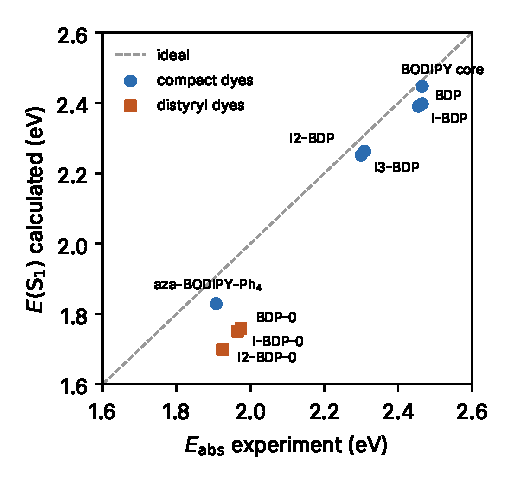
\includegraphics[width=0.48\textwidth]{figures/absorption_parity.pdf}
  \caption{Calculated S$_1$ (TDDFT+$\Delta$SCF) versus experimental absorption energy for the six
  compact dyes (circles) and the three 3,5-distyryl dyes (squares).}
  \label{fig:abs}
\end{figure}

\subsection{Triplet energies, SOC and ISC rates}
\label{sec:isc}

Table~\ref{tab:isc} summarizes the triplet photophysics. The computed S$_1$--T$_1$ gaps of BDP
(0.72~eV) and I2-BDP (0.61~eV) agree with the measured 0.77 and 0.59~eV. For the dyes without heavy
atoms the S$_1$--T$_1$ coupling is below 0.01~cm$^{-1}$ and T$_2$ lies 0.3--0.5~eV above S$_1$, so
$\kisc$ is negligible, in agreement with the absence of measurable ISC. Iodination at the 2,6
positions raises $V_1$ to 13--14~cm$^{-1}$ and gives $\kisc=6.9\times10^{9}$~s$^{-1}$ for I2-BDP
($3.5\times10^{9}$ measured) and $7.1\times10^{9}$~s$^{-1}$ for I3-BDP ($3.9\times10^{9}$ measured),
an overestimate by a factor of about two in both cases. ISC is dominated in both dyes by the
S$_1\to$T$_1$ channel; T$_2$ lies 0.3~eV above S$_1$ and contributes less than $10^{-5}$ of the rate.
Iodine on the meso-phenyl ring alone (I-BDP) gives no significant ISC in the calculation.
\todo{Check whether ref~\citenum{Ly2021} reports $\Phi_T$ or $\kisc$ for I-BDP.}

The MLJ parameters were not fitted. Varying $\lambda_s$ between 0.05 and 0.2~eV and $S$ between 0.5
and 1.2 moves $\kisc$(I2-BDP) between $2.3\times10^{9}$ and $2.8\times10^{10}$~s$^{-1}$
(Table~S\todo{}), so agreement within an order of magnitude, not a factor of two, is what can be
claimed. The ratio $\kisc$(I2-BDP)/$\kisc$(BDP), which is what a screening ranking depends on, is
larger than $10^{11}$ for every parameter set.

\begin{table}
  \caption{Triplet photophysics. $V_1$ is the S$_1$--T$_1$ SOC; rates in s$^{-1}$. Experimental
  values in toluene from ref~\citenum{Ly2021}; ``n.o.'' = not observed.}
  \label{tab:isc}
  \begin{tabular}{lcccccc}
    \toprule
    Dye & $\Delta E_\mathrm{ST}$ calc/exp (eV) & $V_1$ (cm$^{-1}$) & $\kisc$ calc & $\kisc$ exp &
    $\Phi_T$ calc & $\Phi_T$ exp \\
    \midrule
    BODIPY core    & 0.71 / --    & 0.00 & $2\times10^{-2}$ & --  & 0.00 & $\approx0$ \\
    BDP            & 0.72 / 0.77  & 0.00 & $1\times10^{-2}$ & n.o. & 0.00 & n.o. \\
    I-BDP          & 0.72 / 0.76  & 0.00 & 2.9 & -- & 0.00 & -- \\
    I2-BDP         & 0.61 / 0.59  & 13.2 & $6.9\times10^{9}$ & $3.5\times10^{9}$ & 0.95 & 0.84 \\
    I3-BDP         & 0.61 / 0.58  & 13.5 & $7.1\times10^{9}$ & $3.9\times10^{9}$ & 0.95 & 0.81 \\
    aza-BDP-Ph$_4$ & 0.73 / --    & 0.11 & $1.5\times10^{5}$ & -- & 0.00 & low \\
    \midrule
    I2-BDP-0       & 0.50 / --    & 0.43 & $1.7\times10^{7}$ & $4.5\times10^{8}$ & 0.04 & 0.76 \\
    \bottomrule
  \end{tabular}
\end{table}

\subsection{Styryl-extended dyes}
\label{sec:styryl}

The three 3,5-distyryl dyes (BDP-0, I-BDP-0, I2-BDP-0) were computed as (E,E) isomers from a
conformer search, with the same protocol. They are the clearest limitation of the classical
pipeline in this study. Absorption is predicted 77--86~nm (0.21--0.23~eV) too far to the red
(Table~\ref{tab:abs}), and for the diiodo dye I2-BDP-0 the predicted
$\kisc=1.7\times10^{7}$~s$^{-1}$ is 26 times smaller than the measured $4.5\times10^{8}$~s$^{-1}$, so
that $\Phi_T$ is 0.04 instead of 0.76 (Table~\ref{tab:isc}). Conformers do not explain the
discrepancy: across the conformers computed, $\lambda$ varies by 15--18~nm and $\kisc$ by less than a
factor of 1.5.

The numbers point to the $\Delta$SCF step. The error of the uncorrected TDDFT S$_1$ decreases as the
chromophore grows (+0.76~eV for the BODIPY core, +0.23 to +0.27~eV for the distyryl dyes), whereas the
$\Delta$SCF shift stays close to $-0.5$~eV for every dye ($-0.42$ to $-0.77$~eV for the compact dyes,
$-0.46$ to $-0.49$~eV for the distyryl dyes). A correction of nearly constant size, adequate for
compact cyanine-like chromophores, overshoots for extended ones. This diagnosis follows from the
numbers above; we have not tested a remedy, such as a range-separated functional or a correction
that depends on chromophore size. \todo{Update if a range-separated functional or size-dependent
correction is tested.}

The ISC failure has a specific origin that is relevant to the discussion of ISC proxies below. In
the uncorrected TDDFT spectrum of I2-BDP-0, T$_2$ lies only 0.08~eV above S$_1$ and the S$_1$--T$_2$
coupling is 8~cm$^{-1}$; this nearly resonant channel gives $\kisc=1.1\times10^{9}$~s$^{-1}$ and
$\Phi_T=0.67$, close to experiment. Because the $\Delta$SCF correction lowers S$_1$ and T$_1$ but not
the higher triplets, it moves T$_2$ 0.51~eV above S$_1$ and closes that channel, leaving only the
weakly coupled S$_1\to$T$_1$ path ($V_1=0.43$~cm$^{-1}$). The agreement of the uncorrected rate may be
partly fortuitous, since the same calculation places S$_1$ 0.23~eV too high, but it shows that
$\kisc$ in this dye is controlled by the relative position of S$_1$ and an upper triplet to within a
few tenths of an eV. A consistent treatment of all excited states, not a correction of S$_1$ and
T$_1$ alone, is therefore needed for $\pi$-extended dyes.

A methodological note also belongs here. In a first calculation the SMILES strings of these dyes
carried no E/Z labels and the 3D embedding produced cis (Z) styryl groups. Those geometries happened
to give absorption closer to experiment (645--681~nm), an agreement that was meaningless. Because 3D embedding silently assigns an arbitrary configuration to unlabeled double bonds,
any automated screening of $\pi$-extended dyes should specify and verify the stereochemistry; our
pipeline now does both (an automated test checks that the styryl dihedrals are near
\SI{180}{\degree}).

\subsection{Quantum algorithms in small active spaces}

In CAS(4,4) and CAS(6,6) (8 and 12 qubits; 6 and 10 after tapering) the QSVT threshold projection
reproduces the exact dipole weight of the smoothed window to within $10^{-4}$, and the Trotterized
proxy reproduces the exact $V_n$ to three to four significant digits (e.g.\ 27.914 versus
27.915~cm$^{-1}$ for the S$_1$--T$_2$ coupling of I2-BDP), confirming that both algorithms compute
what they are designed to compute.

The values they compute, however, are those of the active-space Hamiltonian. In these active spaces
CASCI places S$_1$ at 259--336~nm for dyes that absorb at 503--650~nm, so the weight in the
700--850~nm window of ref~\citenum{Zhou2025} is zero for every dye, including the aza-BODIPY that
absorbs at 650~nm. Centring the window on the CASCI S$_1$ instead gives weights of 0.6--0.9, which
reflect the active-space spectrum rather than the experimental one.

The ISC proxy at CAS(4,4) does order the dyes by heavy-atom content: the largest S$_1$--T$_n$
coupling over the first three triplets is 0.004--1.4~cm$^{-1}$ without iodine and 28~cm$^{-1}$ for
I2-BDP. Two limitations are visible, though. First, the proxy contains no energy gap, so it cannot
distinguish an open channel from a closed one; in the active space the largest coupling of I2-BDP
is to a triplet that lies above S$_1$, while the classical calculation (and the measured gap) show
that ISC proceeds to T$_1$, 0.6~eV below. Second, when couplings are summed over many triplets as a
figure of merit, the sum for I2-BDP in the classical calculation is dominated by a single high-lying triplet
($\sim$\SI{1100}{cm^{-1}} coupling to T$_5$, 1.5~eV above S$_1$ in the TDDFT spectrum) whose MLJ rate is negligible.
A screening metric based on summed $\lvert V\rvert^2$ would therefore be driven by states that
play no role in the photophysics.

\subsection{Paper-sized active space}

The small active spaces above are far from the 11--45 orbitals considered in
ref~\citenum{Zhou2025}. To test whether a larger active space alone would fix the excitation
energies, we computed CASCI and SC-NEVPT2 at (12e,11o) for the first four dyes
(Table~\ref{tab:cas}, Figure~\ref{fig:cas}). CASCI overestimates S$_1$ by 1.4--2.0~eV. NEVPT2
reduces the error to 0.06--0.27~eV, but its sign changes across dyes ($+0.25$~eV for the BODIPY
core, $-0.27$~eV for I2-BDP); it is larger than the TDDFT+$\Delta$SCF error for two dyes and
comparable for the other two. Since quantum phase estimation on the active-space Hamiltonian would at best reproduce the
CASCI energies, the observables of ref~\citenum{Zhou2025} would require, at minimum, a
dynamic-correlation correction on top of the quantum calculation to be useful for absorption.

\begin{table}
  \caption{S$_1$ excitation energies (eV) in the (12e,11o) active space, def2-SVP, compared with
  experiment and with the classical pipeline.}
  \label{tab:cas}
  \begin{tabular}{lcccc}
    \toprule
    Dye & exp & CASCI & SC-NEVPT2 & TDDFT+$\Delta$SCF \\
    \midrule
    BODIPY core    & 2.46 & 3.97 & 2.71 & 2.45 \\
    BDP            & 2.46 & 4.14 & 2.52 & 2.40 \\
    I2-BDP         & 2.31 & 4.32 & 2.04 & 2.26 \\
    aza-BDP-Ph$_4$ & 1.91 & 3.35 & 1.99 & 1.83 \\
    \bottomrule
  \end{tabular}
\end{table}

\begin{figure}
  \centering
  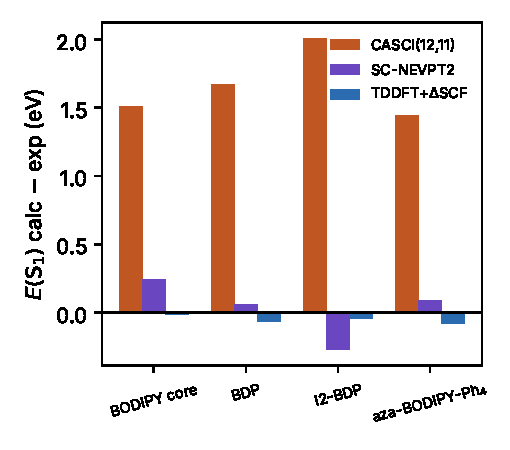
\includegraphics[width=0.48\textwidth]{figures/active_space_error.pdf}
  \caption{Error in the S$_1$ energy for CASCI(12e,11o), SC-NEVPT2 on the same active space, and the
  classical TDDFT+$\Delta$SCF pipeline.}
  \label{fig:cas}
\end{figure}

\subsection{Fault-tolerant resources}

For the (12e,11o) Hamiltonians of I2-BDP and aza-BDP-Ph$_4$, the double-factorization estimate gives
601 logical qubits and $4.4\times10^{7}$ and $4.1\times10^{7}$ Toffoli gates per phase-estimation run,
with one-norms $\lambda$ of 11.5 and 10.8~Ha. The Toffoli count is in the range reported in
ref~\citenum{Zhou2025}; the qubit count is higher than their 180--350, which we attribute to the
different block encoding (double factorization with default parameters here, tensor hypercontraction
there) and to the precision of the rotation registers. \todo{Confirm the source of the qubit-count
difference (DF rank, rotation precision, \texttt{qml.resource} defaults) before stating it.}

% ---------------------------------------------------------------------------------------------
\section{Discussion}

\paragraph{What the quantum observables contribute.} The two algorithms are sound: in simulation they
reproduce the quantities they target. For screening BODIPY photosensitizers, however, the
limiting factor is not the solution of the active-space problem but the physics outside it.
Absorption energies require dynamic correlation, which the active space lacks, and ISC rates require
the singlet--triplet gap and vibronic Franck--Condon factors, which the evolution proxy omits. The
distyryl diiodo dye makes the point sharply: its ISC rate changes by almost two orders of magnitude
depending on whether T$_2$ lies 0.08 or 0.5~eV above S$_1$, a difference to which a gap-free coupling
proxy is blind. A
classical pipeline that costs one to a few CPU-hours per molecule on a few cores already captures the
absorption of compact BODIPYs to within 0.1~eV and their heavy-atom ISC trend within a factor of
two, although it fails for the styryl-extended dyes.

\paragraph{Where quantum algorithms could still help.} The case for quantum computation is stronger
where the classical components used here are unreliable: photosensitizers with transition metals or
open-shell character, where TDDFT and $\Delta$SCF are not trustworthy and static correlation
matters~\cite{Zhou2025}; and couplings between near-degenerate states, where single-reference SOC
is questionable. For such systems the quantum observables should be combined with (i) a dynamic
correlation treatment, for instance perturbation theory on top of quantum-computed reduced density
matrices, and (ii) an energy-resolved ISC observable that includes the gap, e.g.\ a filtered
evolution or a golden-rule estimator with Franck--Condon weights, as in eq~\ref{eq:mlj}. These
extensions, rather than larger active spaces alone, determine whether the quantum observables could
improve on classical screening.

\paragraph{Limitations.} The benchmark is small: nine dyes from essentially one family, and only
three measured ISC rates. One functional and one basis set were used, in the gas phase and at a
single conformer. The internal-conversion rate is fixed from one dye, so fluorescence yields are not
predictions. The MLJ parameters are assumed. The quantum algorithms were run on a simulator with
exactly prepared eigenstates, which removes state-preparation cost and error.

% ---------------------------------------------------------------------------------------------
\section{Conclusions}

We compared the photosensitizer observables proposed for fault-tolerant quantum computers with an
inexpensive classical pipeline and with experiment on BODIPY dyes. The classical pipeline reproduces
absorption to $-0.055\pm0.02$~eV and the heavy-atom enhancement of ISC within a factor of two. The
quantum algorithms work as designed in simulation, but exact active-space energies at the
(12e,11o) level are 1.4--2.0~eV too high, and the ISC proxy lacks the energy gap that determines
which channel is active. For this class of molecules, a quantum advantage in screening would require
dynamic correlation and vibronic effects on top of the quantum calculation, and is most likely to
appear for metal-containing or strongly correlated photosensitizers. The classical pipeline itself
does not transfer to $\pi$-extended styryl dyes, where the $\Delta$SCF correction overshoots S$_1$ by
about 0.2~eV and closes a near-resonant S$_1\to$T$_2$ ISC channel; these dyes are a demanding test for
any method, classical or quantum, because their ISC depends on the S$_1$--T$_2$ gap at the 0.1~eV
level.

% ---------------------------------------------------------------------------------------------
\begin{acknowledgement}
\todo{Funding and computing resources.}
\end{acknowledgement}

\begin{suppinfo}
\todo{Geometries (xyz), per-dye JSON outputs, MLJ sensitivity table, CAS(4,4)/(6,6) quantum results,
singlet-window check, screening of heavy-atom candidates.}
\end{suppinfo}

\section*{Data Availability}
Code, geometries and all results: \url{https://github.com/pifparfait/psscreen}. \todo{Archive a
tagged release on Zenodo and cite the DOI.}

\bibliography{refs}

\end{document}
